\section{Suggested textbook practice: Section 12.2}\label{textbook}
These are the 13 suggested exercises from \emph{Calculus, Eighth Edition}, Section 12.2. Question numbers, shared instructions, and diagrams have been checked against the supplied textbook. Source figures are reproduced below so that the questions are self-contained. Solution sketches are schematic where the original question gives no numerical scale.

\subsection{12.2, Exercise 1: point membership}
\paragraph{Question.} Which of (I)--(IV) lie on the graph of the function $z=f(x,y)$, where $f(x,y)=-3$?
\[
\mathrm{I}:(1,0,1),\quad \mathrm{II}:(\sqrt8,1,3),\quad
\mathrm{III}:(-3,7,-3),\quad \mathrm{IV}:(1,1,1/2).
\]
\paragraph{Necessary work.} See \hyperref[graph]{graphs and point membership}. Every graph point must have third coordinate $-3$.
\paragraph{Answer.} Only \textbf{III}, $(-3,7,-3)$.

\subsection{12.2, Exercise 3: point membership}
\paragraph{Question.} Which of (I)--(IV) lie on the graph of the function $z=f(x,y)$, where $f(x,y)=1/(x^2+y^2)$?
\[
\mathrm{I}:(1,0,1),\quad \mathrm{II}:(\sqrt8,1,3),\quad
\mathrm{III}:(-3,7,-3),\quad \mathrm{IV}:(1,1,1/2).
\]
\paragraph{Necessary work.} At their respective input pairs, $f$ equals $1,1/9,1/58,1/2$. Compare each with its proposed third coordinate. The origin is excluded from the domain, but none of these inputs is the origin. See \hyperref[graph]{graph membership}.
\paragraph{Answer.} \textbf{I and IV}.

\subsection{12.2, Exercise 5: match surfaces}
\paragraph{Question.} Without a calculator or computer, match the functions with their graphs in Figure 12.27.
\[
\begin{array}{ll}
\text{(a) }z=2+x^2+y^2,&\text{(b) }z=2-x^2-y^2,\\
\text{(c) }z=2(x^2+y^2),&\text{(d) }z=2+2x-y,\\
\text{(e) }z=2.&
\end{array}
\]
\begin{center}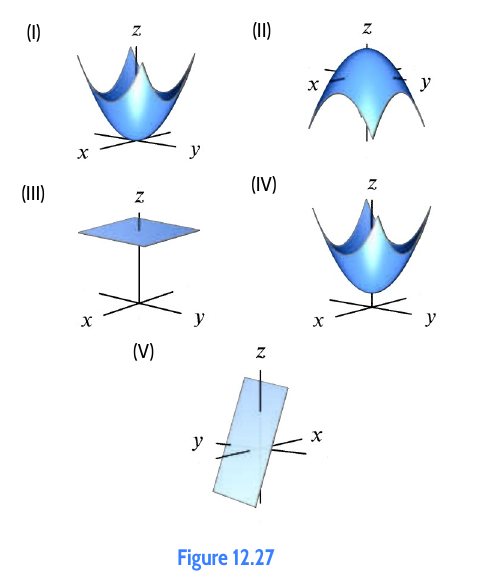
\includegraphics[width=.58\linewidth]{graphs/source-12-2-5.png}\end{center}
\paragraph{Necessary work.} Use \hyperref[transform]{graph transformations}: (a) has an upward vertex above the origin; (b) opens downward; (c) has its upward vertex at the origin; (d) is a tilted plane; (e) is horizontal.
\paragraph{Answer.} (a) IV; (b) II; (c) I; (d) V; (e) III.

\subsection{12.2, Exercise 7: read cross-sections}
\paragraph{Question.} Figure 12.29 shows the graph of $z=f(x,y)$.
\begin{enumerate}
\item[(a)] Suppose $y$ is fixed and positive. Does $z$ increase or decrease as $x$ increases? Graph $z$ against $x$.
\item[(b)] Suppose $x$ is fixed and positive. Does $z$ increase or decrease as $y$ increases? Graph $z$ against $y$.
\end{enumerate}
\begin{center}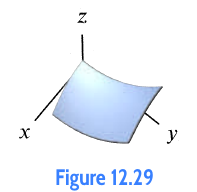
\includegraphics[width=.28\linewidth]{graphs/source-12-2-7.png}\end{center}
\paragraph{Necessary work.} Follow the surface parallel to the indicated input axis; keep the other input fixed. See \hyperref[cross]{cross-sections}. The perspective drawing must be read using its labelled axes.
\paragraph{Answer.} (a) $z$ decreases as $x$ increases; the pictured section bends downward. (b) $z$ increases as $y$ increases; the pictured section bends upward. The following sketches convey shape, not numerical data.
\begin{center}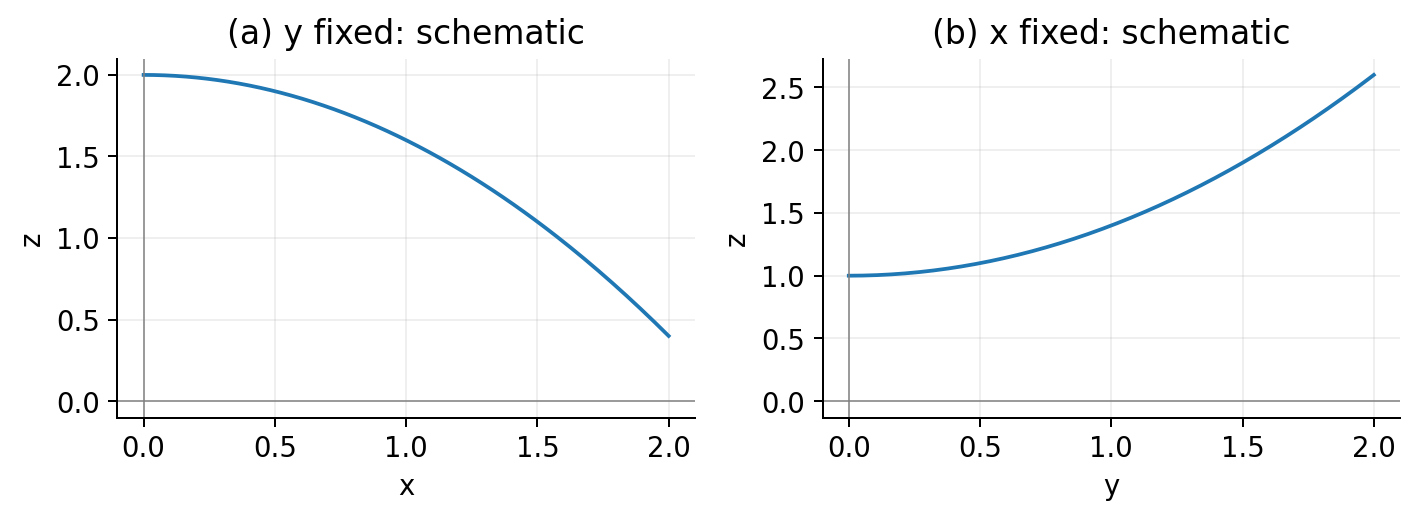
\includegraphics[width=.88\linewidth]{graphs/answer-12-2-7.png}\end{center}

\subsection{12.2, Exercise 9: sphere}
\paragraph{Question.} Sketch a graph of the surface and briefly describe it in words: $x^2+y^2+z^2=9$.
\paragraph{Necessary work.} The sum of squared distances from the origin is $3^2$. Coordinate-plane traces are circles of radius $3$. See \hyperref[graph]{surfaces and the vertical-line test}.
\paragraph{Answer.} A sphere centered at $(0,0,0)$ with radius $3$; axis intercepts are $(\pm3,0,0),(0,\pm3,0),(0,0,\pm3)$. The whole sphere is not the graph of one function $z=f(x,y)$. Its sketch appears in the four-panel figure after Exercise 15.

\subsection{12.2, Exercise 11: downward paraboloid}
\paragraph{Question.} Sketch a graph of the surface and briefly describe it in words: $z=5-x^2-y^2$.
\paragraph{Necessary work.} Reflect $x^2+y^2$ vertically and translate upward by $5$; see \hyperref[transform]{transformations}. Vertical traces are downward parabolas, and horizontal traces satisfy $x^2+y^2=5-c$.
\paragraph{Answer.} A downward-opening circular paraboloid with vertex $(0,0,5)$ and vertical axis. Its intersection with $z=0$ is the circle of radius $\sqrt5$. See the sketch after Exercise 15.

\subsection{12.2, Exercise 13: plane}
\paragraph{Question.} Sketch a graph of the surface and briefly describe it in words: $2x+4y+3z=12$.
\paragraph{Necessary work.} Set two coordinates to zero in turn. Equivalently, $x/6+y/3+z/4=1$. See \hyperref[plane]{planes}.
\paragraph{Answer.} A plane with intercepts $(6,0,0),(0,3,0),(0,0,4)$, or $z=4-\frac23x-\frac43y$. The triangular first-octant patch in the figure is part of an infinite plane.

\subsection{12.2, Exercise 15: cylinder}
\paragraph{Question.} Sketch a graph of the surface and briefly describe it in words: $x^2+z^2=4$.
\paragraph{Necessary work.} Each plane $y=b$ cuts the same circle of radius $2$ in $xz$ coordinates. The missing variable is $y$; see \hyperref[cylinder]{cylinders}.
\paragraph{Answer.} A circular cylinder of radius $2$, centered on and extending in both directions along the $y$-axis. The whole cylinder is not a graph $z=f(x,y)$.
\begin{center}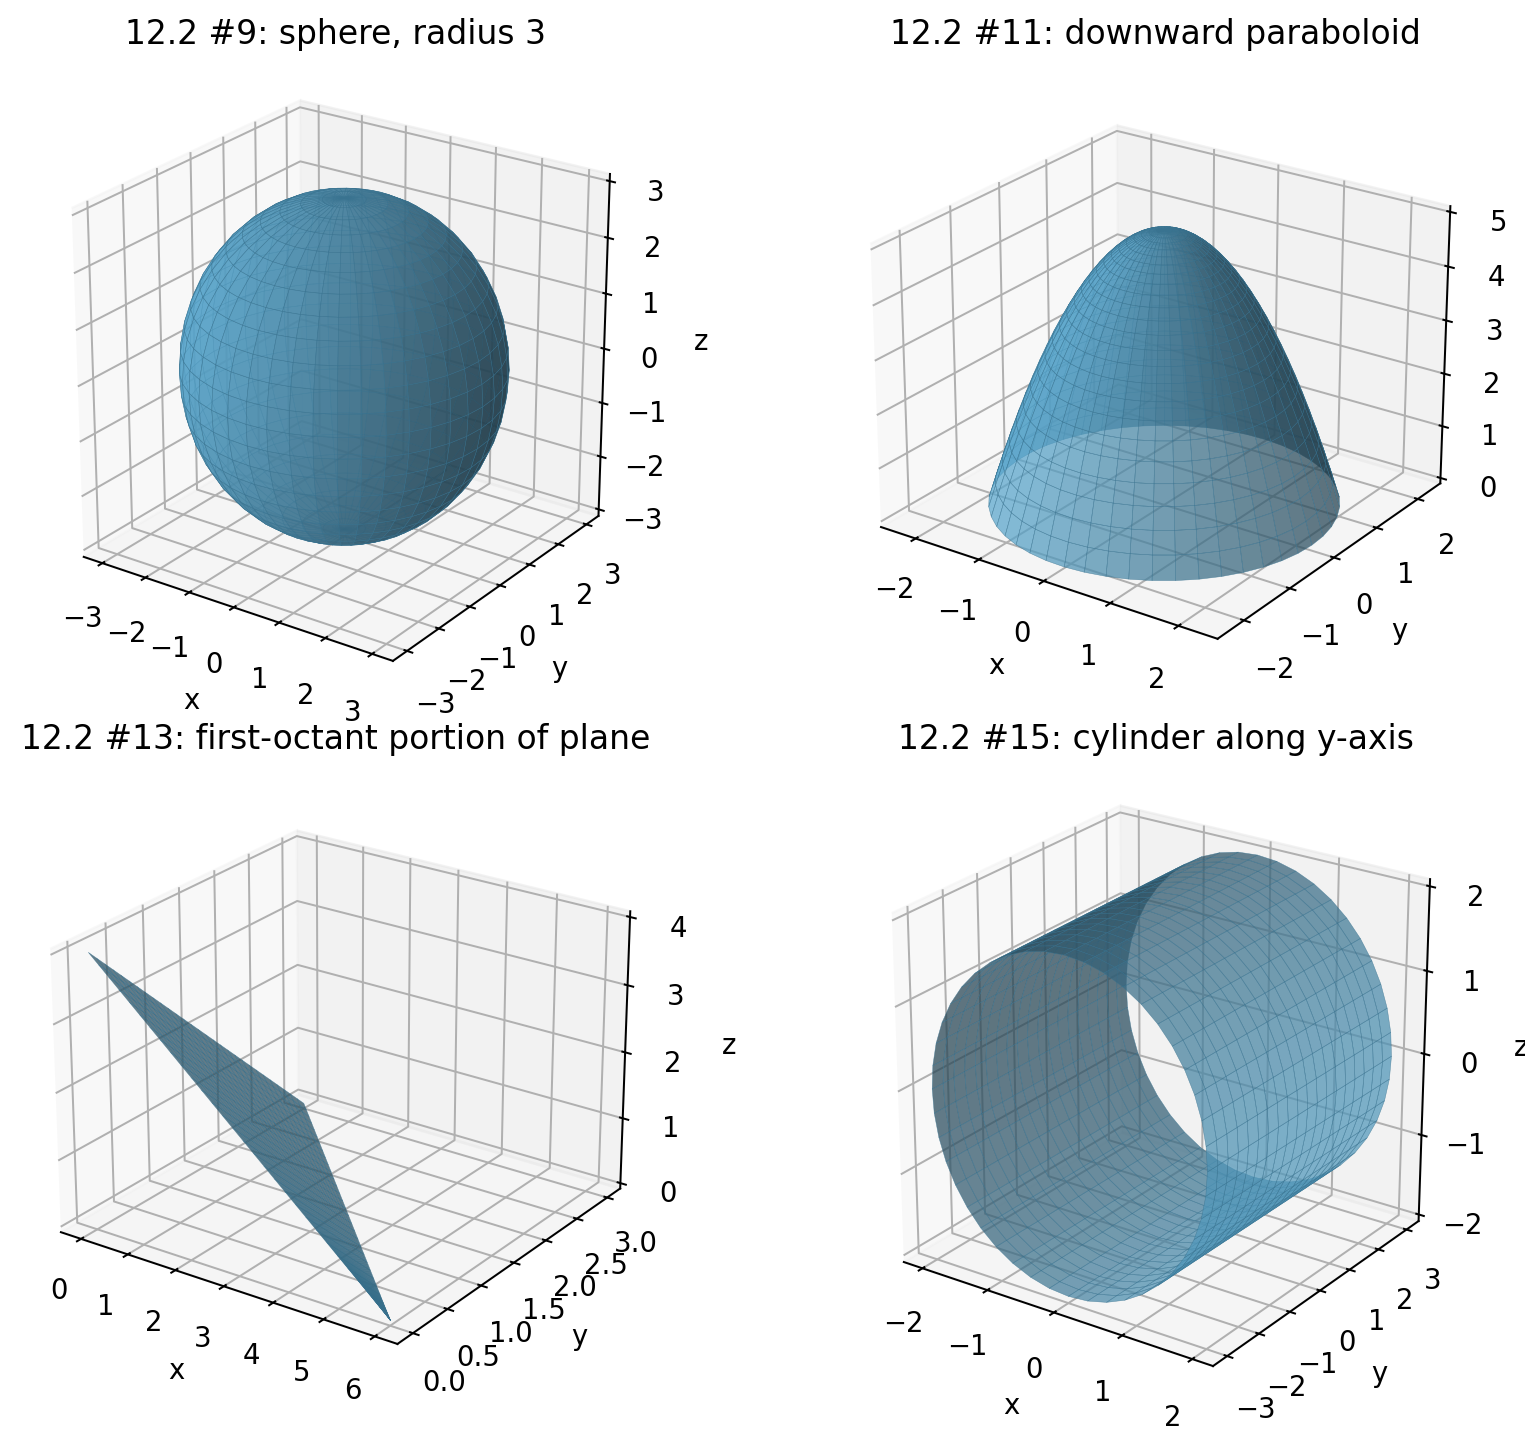
\includegraphics[width=.96\linewidth]{graphs/answer-12-2-surfaces.png}\end{center}

\subsection{12.2, Exercise 17: translate a sphere}
\paragraph{Question.} Find the equation of the surface: a sphere of radius $3$ centered at $(0,\sqrt7,0)$.
\paragraph{Necessary work.} The distance from $(x,y,z)$ to the given center is $3$; square the distance equation. See \hyperref[graph]{surface equations}.
\paragraph{Answer.} $\boxed{x^2+(y-\sqrt7)^2+z^2=9}$.

\subsection{12.2, Exercise 21: drug concentration}
\paragraph{Question.} The concentration $C$, in mg/liter, of a drug in the blood is a function of $x$, the amount in mg of the drug given, and $t$, the time in hours since injection. For $0\le x\le4$ and $t\ge0$,
\[C=f(x,t)=te^{-t(5-x)}.\]
Graph the following single-variable functions and explain their significance in terms of drug concentration: (a) $f(4,t)$; (b) $f(x,1)$.
\paragraph{Necessary work.} Substitute the fixed input, as in \hyperref[cross]{cross-sections}:
\[
f(4,t)=te^{-t}\quad(t\ge0),\qquad f(x,1)=e^{x-5}\quad(0\le x\le4).
\]
For (a), $\frac{d}{dt}(te^{-t})=e^{-t}(1-t)$, so the maximum is $1/e$ at $t=1$. For (b), the exponential is increasing and convex.
\paragraph{Answer.} (a) After a $4$ mg injection, concentration starts at $0$, peaks at $1/e\approx0.368$ mg/liter after $1$ hour, then approaches $0$. (b) One hour after injection, concentration increases from $e^{-5}$ to $e^{-1}$ mg/liter as dose increases from $0$ to $4$ mg. These are interpretations of the stated mathematical model.
\begin{center}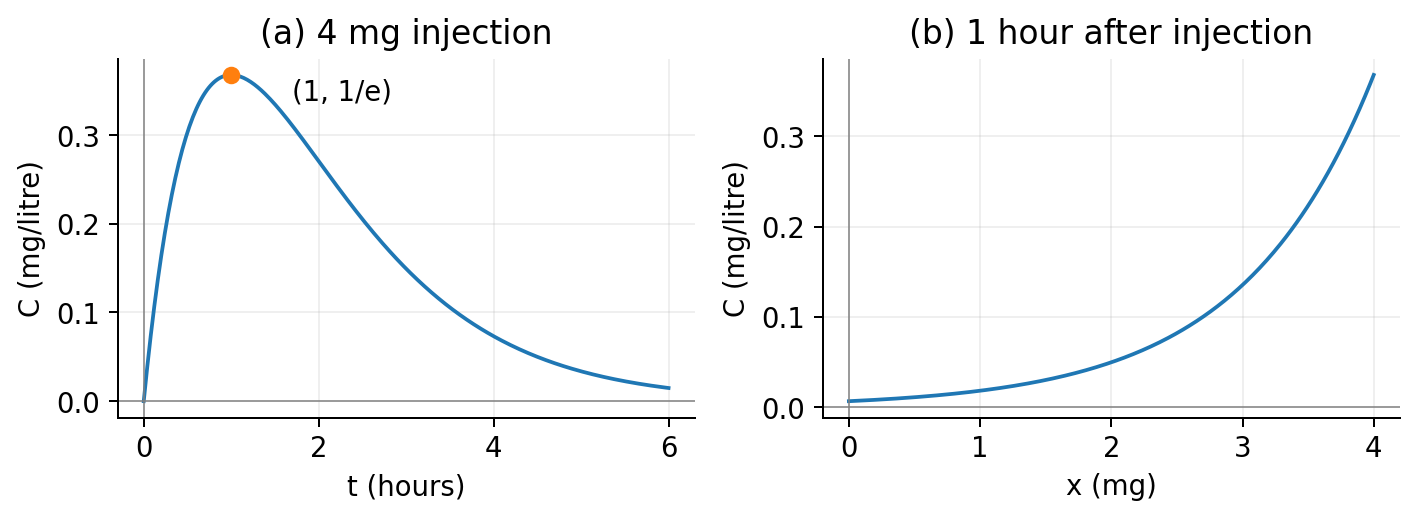
\includegraphics[width=.9\linewidth]{graphs/answer-12-2-21.png}\end{center}

\subsection{12.2, Exercise 27: identify the fixed variable}
\paragraph{Question.} Without a calculator or computer, for $z=x^2+2xy^2$, determine which of (I)--(II) in Figure 12.30 are cross-sections with $x$ fixed and which are cross-sections with $y$ fixed.
\begin{center}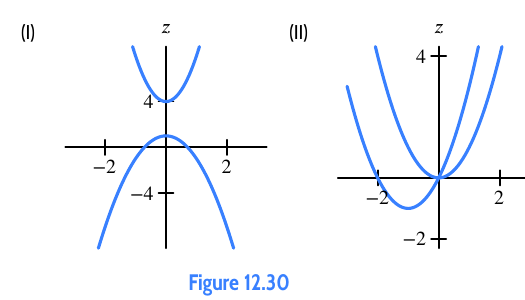
\includegraphics[width=.72\linewidth]{graphs/source-12-2-27.png}\end{center}
\paragraph{Necessary work.} With $x=a$, $z=a^2+2ay^2$: parabolas are symmetric about $y=0$, opening upward for $a>0$ and downward for $a<0$. With $y=b$, $z=x^2+2b^2x=(x+b^2)^2-b^4$: all open upward, pass through $(0,0)$, and have vertices $(-b^2,-b^4)$. See \hyperref[cross]{cross-section families}.
\paragraph{Answer.} I has $x$ fixed; II has $y$ fixed.

\subsection{12.2, Exercise 31: match cross-section families}
\paragraph{Question.} Without a calculator or computer, match the functions with their cross-sections with $x$ fixed in Figure 12.31:
\[
\begin{array}{ll}
\text{(a) }z=1/(1+x^2+y^2),&\text{(b) }z=1+x+y,\\
\text{(c) }z=e^{-x+y},&\text{(d) }z=e^{x-y},\\
\text{(e) }z=\sin(xy),&\text{(f) }z=x^2.
\end{array}
\]
\begin{center}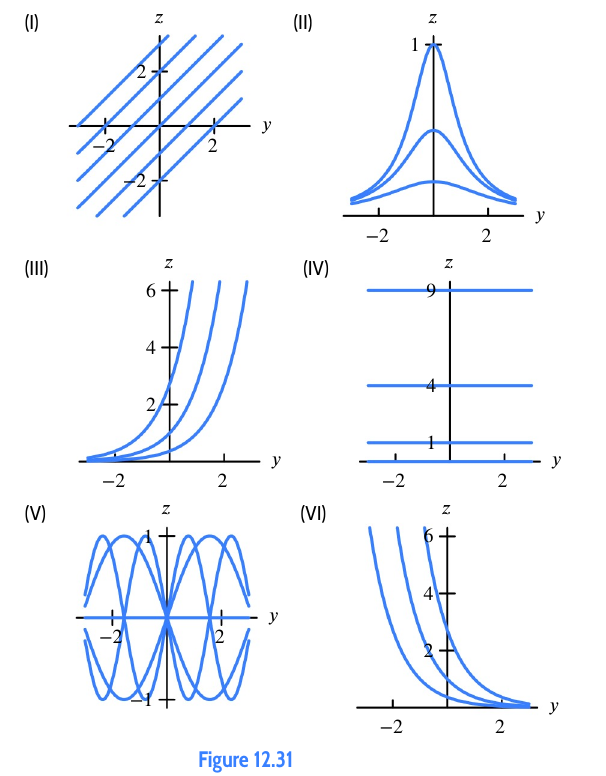
\includegraphics[width=.73\linewidth]{graphs/source-12-2-31.png}\end{center}
\paragraph{Necessary work.} Set $x=a$; see \hyperref[cross]{cross-sections}. The families are, respectively: positive symmetric humps $1/(1+a^2+y^2)$; lines of slope $1$; increasing exponentials $e^{-a}e^y$; decreasing exponentials $e^ae^{-y}$; sines of variable frequency $\sin(ay)$; horizontal lines $z=a^2$.
\paragraph{Answer.} (a) II; (b) I; (c) III; (d) VI; (e) V; (f) IV.

\subsection{12.2, Exercise 41: travelling wave}
\paragraph{Question.} A wave travels along a canal. Let $x$ be the distance along the canal, $t$ be the time, and $z$ be the height of the water above the equilibrium level. The graph of $z$ as a function of $x$ and $t$ is in Figure 12.33.
\begin{enumerate}
\item[(a)] Draw the profile of the wave for $t=-1,0,1,2$. (Put the $x$-axis to the right and the $z$-axis vertical.)
\item[(b)] Is the wave traveling in the direction of increasing or decreasing $x$?
\item[(c)] Sketch a surface representing a wave traveling in the opposite direction.
\end{enumerate}
\begin{center}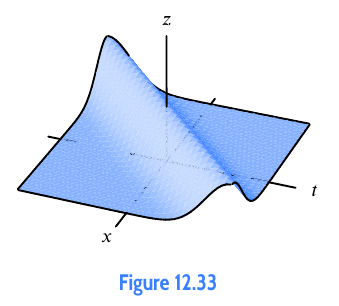
\includegraphics[width=.48\linewidth]{graphs/source-12-2-41.png}\end{center}
\paragraph{Necessary work.} Use \hyperref[cross]{cross-sections} with time fixed. Follow the ridge as $t$ increases: the crest moves toward larger $x$. A schematic translating pulse has the form $z=g(x-vt)$ with $v>0$; reversing time gives $g(x+vt)$. The diagram provides no numerical speed or precise formula.
\paragraph{Answer.} (a) The four hump-shaped profiles shift right as time increases, as sketched below. (b) Increasing $x$. (c) Reverse the ridge direction; the second sketch uses $g(s)=e^{-s^2}$ purely to illustrate a wave moving toward decreasing $x$.
\begin{center}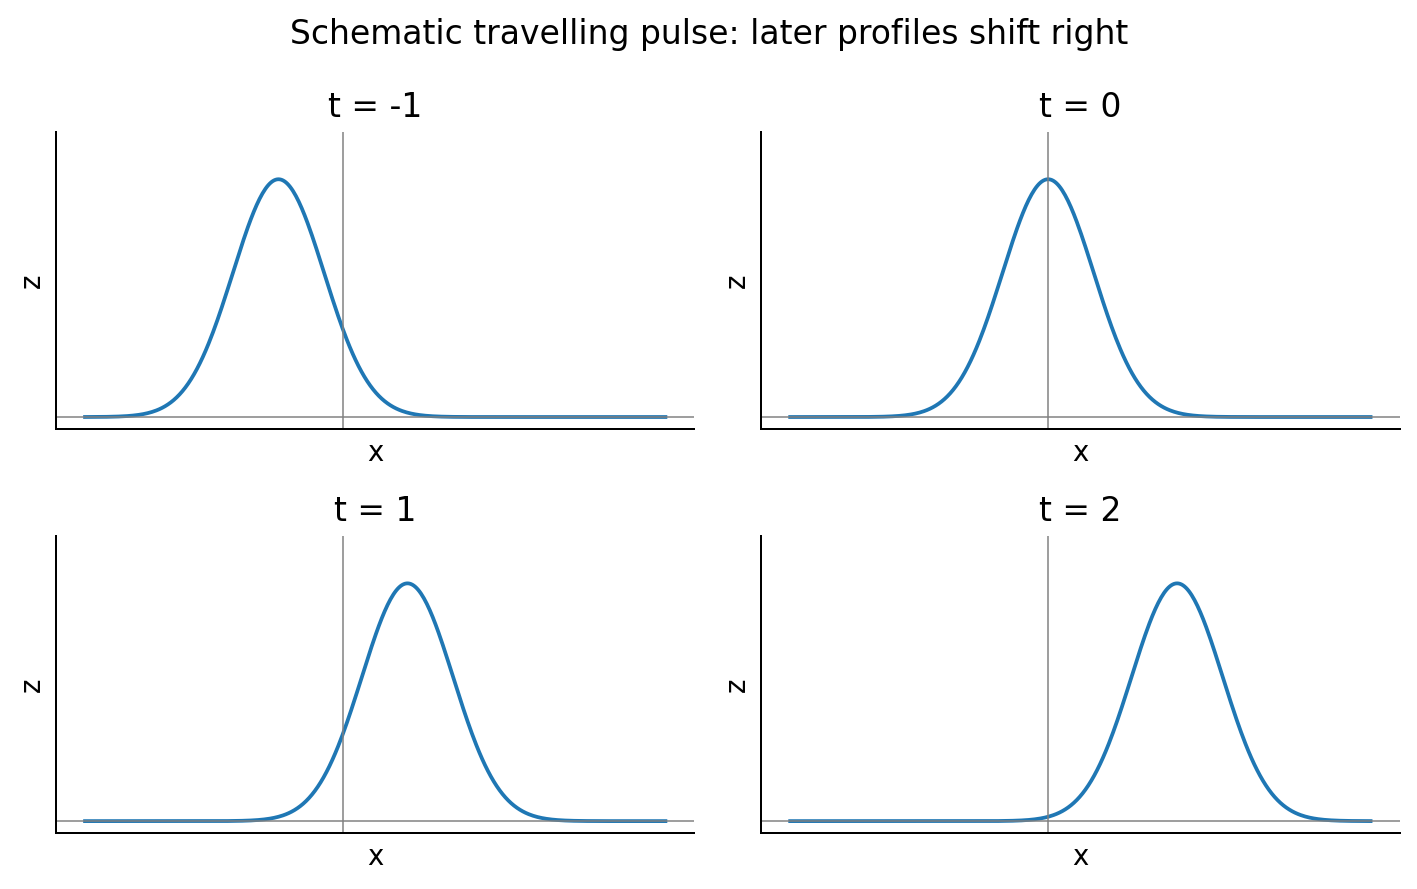
\includegraphics[width=.88\linewidth]{graphs/answer-12-2-41.png}\end{center}
\begin{center}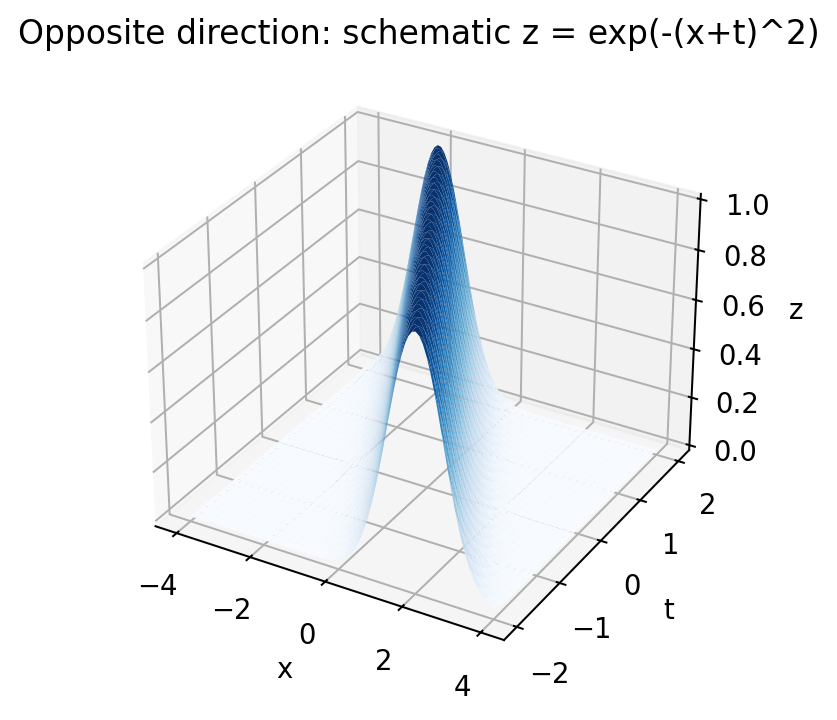
\includegraphics[width=.62\linewidth]{graphs/answer-12-2-41c.png}\end{center}

\section{Suggested textbook practice: Section 12.3}
The following 13 exercises complete the supplied suggested-exercise list. All contour values shown on solution figures are function values, rather than radii.

\subsection{12.3, Exercise 1: surface to contours}
\paragraph{Question.} Sketch a possible contour diagram for the surface below, marked with reasonable $z$-values. (Note: There are many possible answers.)
\begin{center}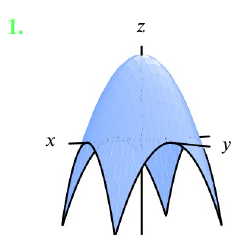
\includegraphics[width=.35\linewidth]{graphs/source-12-3-1.png}\end{center}
\paragraph{Necessary work.} The surface is a downward bowl. Horizontal slices project to concentric circles, with larger heights nearer the center; see \hyperref[contour]{contours}. One model consistent with its shape is $z=4-x^2-y^2$.
\paragraph{Answer.} A valid diagram has center value $4$ and circles $x^2+y^2=4-c$ labelled $c=3,2,1,0$ from inside outward. The particular heights are a reasonable choice, not measurements from the source.
\begin{center}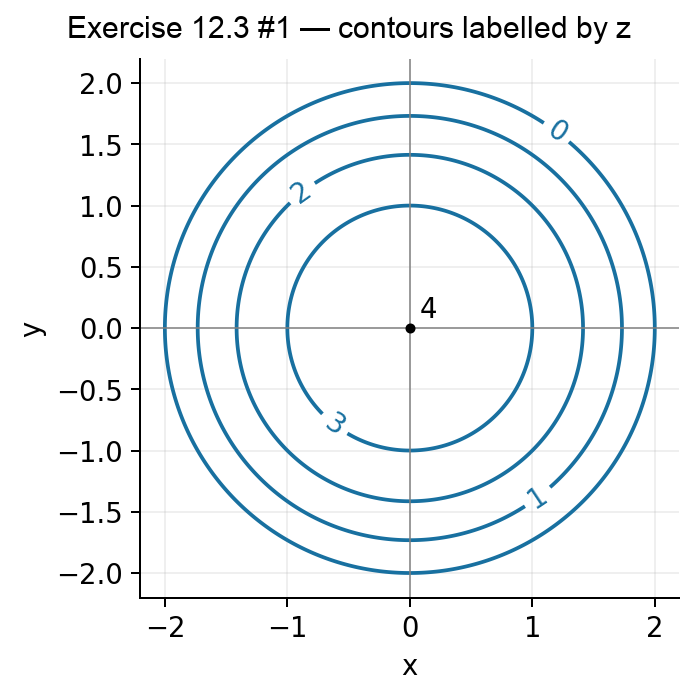
\includegraphics[width=.51\linewidth]{graphs/answer-12-3-1.png}\end{center}

\subsection{12.3, Exercise 3: a circular depression}
\paragraph{Question.} Sketch a possible contour diagram for the surface below, marked with reasonable $z$-values. (Note: There are many possible answers.)
\begin{center}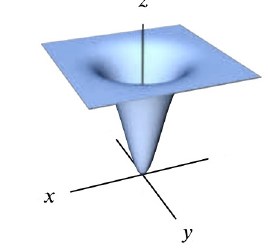
\includegraphics[width=.36\linewidth]{graphs/source-12-3-3.png}\end{center}
\paragraph{Necessary work.} The center is low and the surface rises outward while flattening. Thus choose concentric circles whose values increase outward; see \hyperref[contour]{contour interpretation}. For a concrete illustration, $z=4(1-e^{-(x^2+y^2)})$ has this qualitative shape. Its level $c$ has radius $\sqrt{-\ln(1-c/4)}$, for $0<c<4$.
\paragraph{Answer.} The labelled circles below give one possible answer. Their labels increase from $1$ through $2,3,3.5$; the center has height $0$ in this illustrative model. Other reasonable numerical choices are valid. These levels are not equally spaced, so do not compare their gaps as if their height increments were equal.
\begin{center}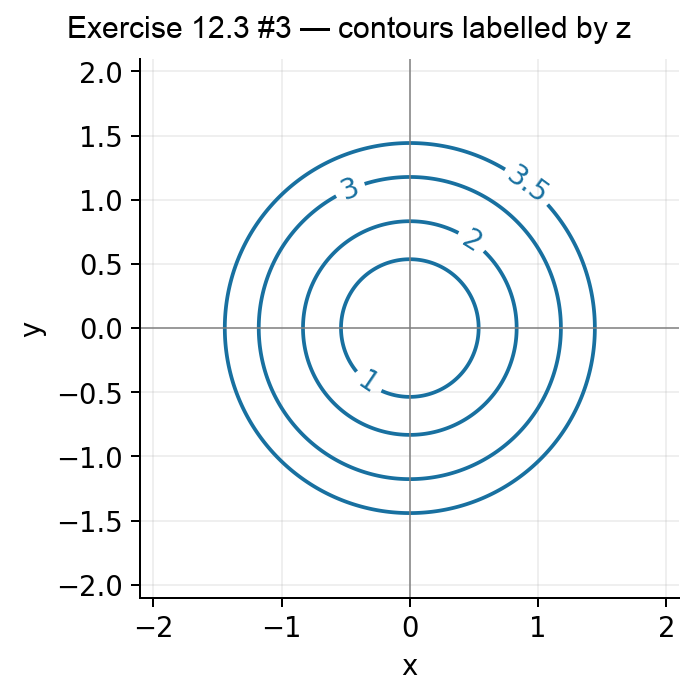
\includegraphics[width=.51\linewidth]{graphs/answer-12-3-3.png}\end{center}

\subsection{12.3, Exercise 5: read a contour value}
\paragraph{Question.} Use the contour diagram of $f(x,y)$ given in Figure 12.52 to find $f(1,3)$.
\begin{center}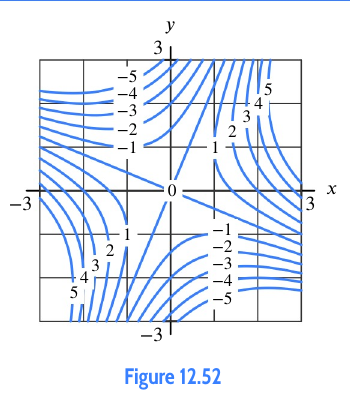
\includegraphics[width=.53\linewidth]{graphs/source-12-3-5.png}\end{center}
\paragraph{Necessary work.} Locate $(1,3)$ and follow its curve to the label $-1$; see \hyperref[estimate]{reading contour values}. Do not confuse the nearby sloping zero contour with the curve through this point.
\paragraph{Answer.} $\boxed{f(1,3)=-1}$.

\subsection{12.3, Exercise 7: find a point on a level set}
\paragraph{Question.} Use the contour diagram of $f(x,y)$ given in Figure 12.52 to find a point where $f(x,y)=0$.
\begin{center}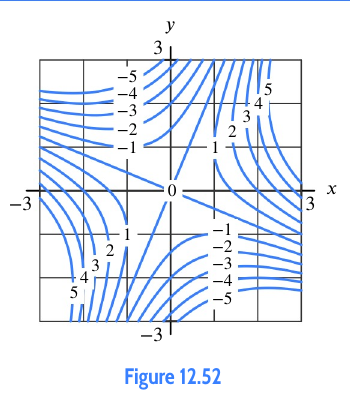
\includegraphics[width=.45\linewidth]{graphs/source-12-3-5.png}\end{center}
\paragraph{Necessary work.} Choose a point on a contour labelled $0$; see \hyperref[contour]{level sets}. The origin lies on that level set.
\paragraph{Answer.} $(0,0)$; other points on the zero contour are also valid.

\subsection{12.3, Exercise 9: contour through a point}
\paragraph{Question.} Let $f(x,y)=3x^2y+7x+20$. Find an equation for the contour that goes through the point $(5,10)$.
\paragraph{Necessary work.} First find the output at the point: $f(5,10)=3(25)(10)+35+20=805$. Then set the function equal to that value; see \hyperref[contour]{finding contours algebraically}.
\paragraph{Answer.} $\boxed{3x^2y+7x+20=805}$. Equivalently $y=(785-7x)/(3x^2)$, with $x\ne0$.

\subsection{12.3, Exercise 11: match surfaces and contour diagrams}
\paragraph{Question.} Match the surfaces (a)--(e) in Figure 12.53 with the contour diagrams (I)--(V) in Figure 12.54.
\begin{center}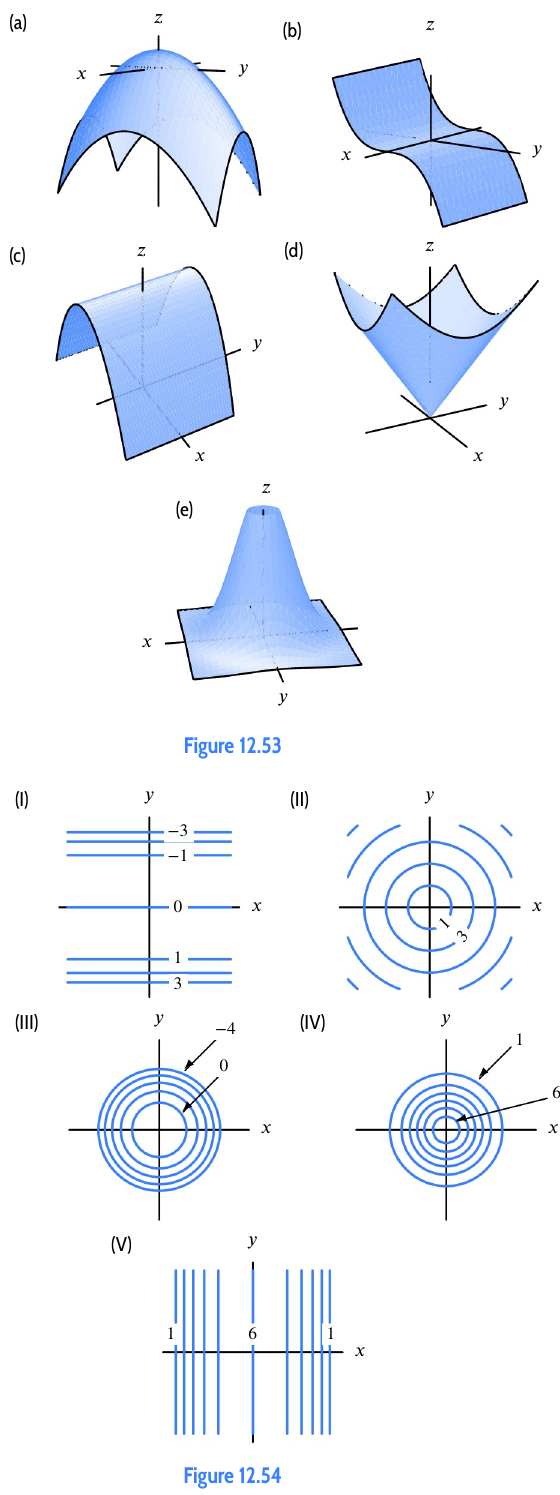
\includegraphics[height=.70\textheight,keepaspectratio]{graphs/source-12-3-11.png}\end{center}
\paragraph{Necessary work.} Use both shape and labels; see \hyperref[contour]{contour interpretation}. Surface (a) is a downward radial bowl. Surface (b) is a trough: its height is smallest on the central line and rises in either $y$ direction, producing paired horizontal contours. Surface (c) is a downward parabolic cylinder with a maximum along its central ridge and no change parallel to $y$, producing paired vertical contours. Surface (d) is an upward cone; (e) is a high central radial mound.
\paragraph{Answer.} (a) III (circle values decrease outward); (b) I (horizontal lines with values decreasing as $y$ increases); (c) V (vertical paired lines); (d) II (evenly spaced circles); (e) IV (circle values highest near the center).

\subsection{12.3, Exercise 13: tables to contour diagrams}
\paragraph{Question.} Match Tables 12.6--12.9 with contour diagrams (I)--(IV) in Figure 12.56. The four tables and all four candidate diagrams are reproduced here.
\begin{center}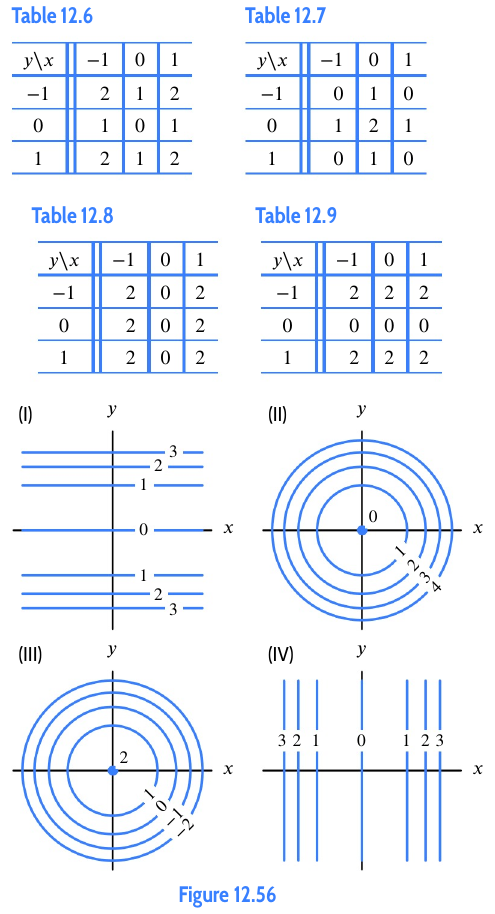
\includegraphics[width=.62\linewidth]{graphs/source-12-3-13.png}\end{center}
\paragraph{Necessary work.} See \hyperref[table]{tables and contours}. Table 12.6 has a central minimum, consistent with $x^2+y^2$. Table 12.7 has a central maximum, consistent with $2-x^2-y^2$. In Table 12.8 the entries depend only on $x$; in Table 12.9 they depend only on $y$. The corresponding vertical or horizontal lines must also have the matching labels. These simple formulas explain the matches; a finite table alone does not uniquely determine a function everywhere.
\paragraph{Answer.} Table 12.6 $\to$ II; Table 12.7 $\to$ III; Table 12.8 $\to$ IV; Table 12.9 $\to$ I.

\subsection{12.3, Exercise 15: parallel line contours}
\paragraph{Question.} Sketch a contour diagram for $f(x,y)=3x+3y$ with at least four labeled contours. Describe in words the contours and how they are spaced.
\paragraph{Necessary work.} Set $3x+3y=c$, giving $y=-x+c/3$; see \hyperref[contour]{algebraic contours}. Choose, for example, $c=-6,-3,0,3,6$.
\paragraph{Answer.} Parallel lines of slope $-1$, equally spaced for equally spaced values of $c$. A level change $\Delta c$ gives perpendicular separation $|\Delta c|/(3\sqrt2)$; for $\Delta c=3$, this is $1/\sqrt2$.
\begin{center}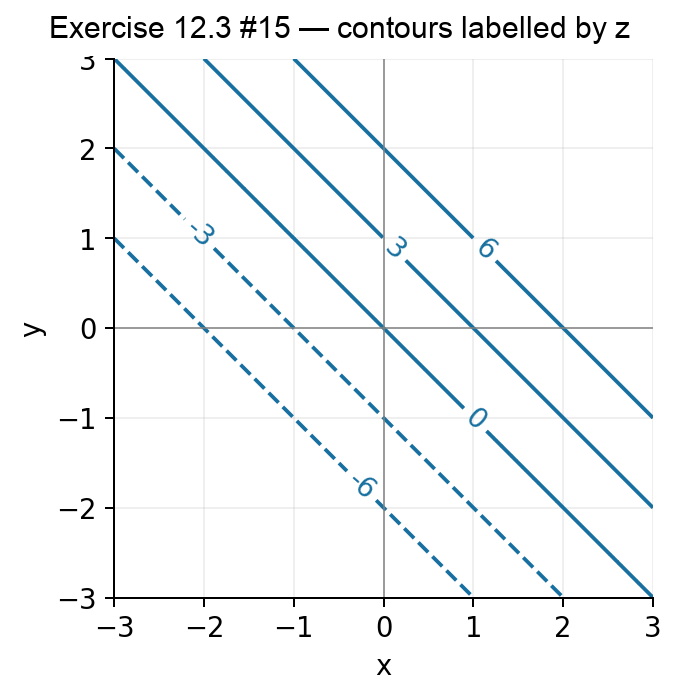
\includegraphics[width=.51\linewidth]{graphs/answer-12-3-15.png}\end{center}

\subsection{12.3, Exercise 17: downward bowl contours}
\paragraph{Question.} Sketch a contour diagram for $f(x,y)=-x^2-y^2+1$ with at least four labeled contours. Describe in words the contours and how they are spaced.
\paragraph{Necessary work.} The level equation is $x^2+y^2=1-c$. Levels exist only for $c\le1$; see \hyperref[contour]{circular contours}. Use $c=0,-1,-2,-3$, whose radii are $1,\sqrt2,\sqrt3,2$.
\paragraph{Answer.} Concentric circles centered at the origin, with decreasing labels outward. For equal decreases in $c$, successive circles get closer together farther from the center, indicating increasing steepness. The $c=1$ level is the origin alone.
\begin{center}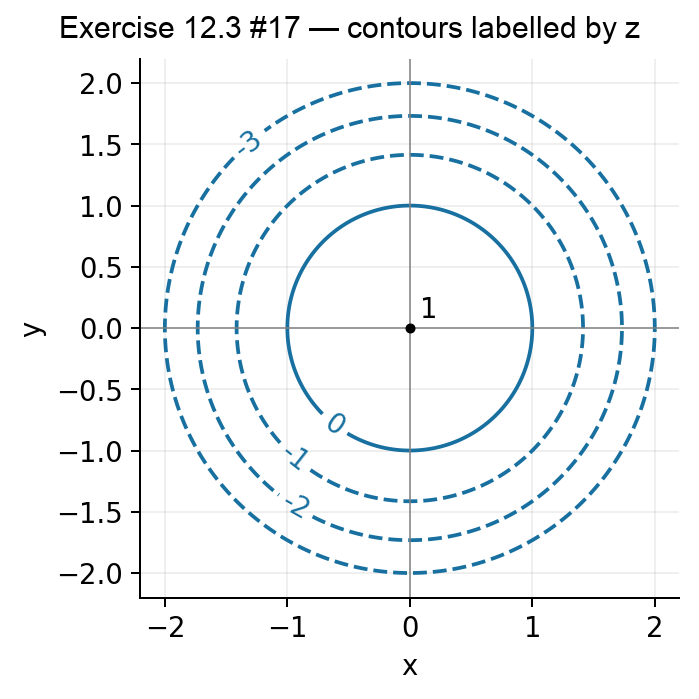
\includegraphics[width=.51\linewidth]{graphs/answer-12-3-17.png}\end{center}

\subsection{12.3, Exercise 19: parabolic contours}
\paragraph{Question.} Sketch a contour diagram for $f(x,y)=y-x^2$ with at least four labeled contours. Describe in words the contours and how they are spaced.
\paragraph{Necessary work.} Set $y-x^2=c$, so $y=x^2+c$. Choose $c=-2,-1,0,1,2$; see \hyperref[contour]{algebraic contours}.
\paragraph{Answer.} Upward-opening parabolas with vertices $(0,c)$, translated vertically. For equal increments of $c$, the vertical separation at fixed $x$ is constant. Their perpendicular separation is not constant; the curves become closer in the transverse direction as $|x|$ grows.
\begin{center}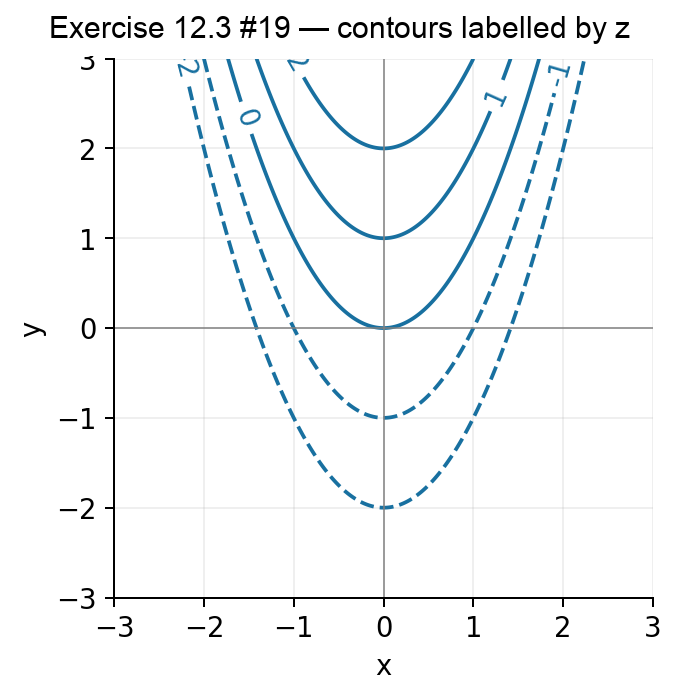
\includegraphics[width=.51\linewidth]{graphs/answer-12-3-19.png}\end{center}

\subsection{12.3, Exercise 25: interpret contour labels}
\paragraph{Question.} Each contour diagram (a)--(c) in Figure 12.59 shows satisfaction with quantities of two items $X$ and $Y$ combined. Match (a)--(c) with the items in (I)--(III):
\begin{enumerate}
\item[(I)] $X$: Income; $Y$: Leisure time.
\item[(II)] $X$: Income; $Y$: Hours worked.
\item[(III)] $X$: Hours worked; $Y$: Time spent commuting.
\end{enumerate}
\begin{center}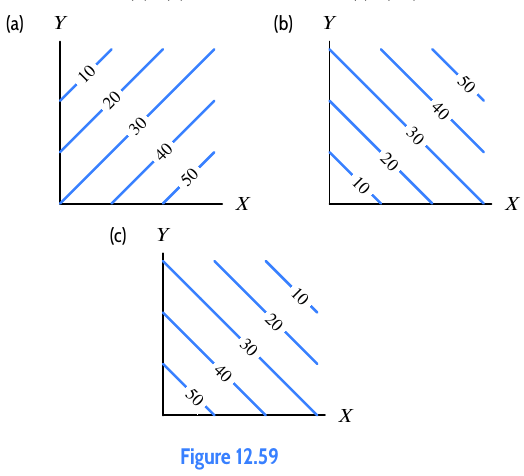
\includegraphics[width=.67\linewidth]{graphs/source-12-3-25.png}\end{center}
\paragraph{Necessary work.} Track whether the labels increase or decrease on moving right and upward; see \hyperref[estimate]{reading contour diagrams}. In (a), increasing $X$ raises satisfaction but increasing $Y$ lowers it. In (b), increasing either quantity raises satisfaction. In (c), increasing either quantity lowers satisfaction. Use the preferences represented by this question's model.
\paragraph{Answer.} (a) II; (b) I; (c) III.

\subsection{12.3, Exercise 27: trade-off along a contour}
\paragraph{Question.} Figure 12.61 shows a contour diagram of Dan's happiness with snacks of different numbers of cherries and grapes. (a) What is the slope of the contours? (b) What does the slope tell you?
\begin{center}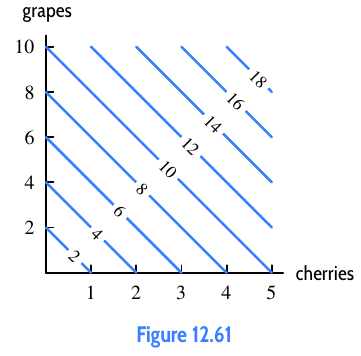
\includegraphics[width=.50\linewidth]{graphs/source-12-3-27.png}\end{center}
\paragraph{Necessary work.} On a fixed contour, increasing cherries by $1$ decreases grapes by $2$. Thus
\[\frac{\Delta(\text{grapes})}{\Delta(\text{cherries})}=-2.\]
See \hyperref[contour]{constant-output trade-offs}.
\paragraph{Answer.} (a) $-2$ grapes per cherry. (b) Replacing two grapes with one cherry leaves Dan's happiness unchanged in this model; conversely, he needs two additional grapes to compensate for one fewer cherry.

\subsection{12.3, Exercise 47: profit contours}
\paragraph{Question.} A manufacturer sells two goods, one at a price of \$3000 a unit and the other at a price of \$12,000 a unit. A quantity $q_1$ of the first good and $q_2$ of the second good are sold at a total cost of \$4000 to the manufacturer.
\begin{enumerate}
\item[(a)] Express the manufacturer's profit, $\pi$, as a function of $q_1$ and $q_2$.
\item[(b)] Sketch curves of constant profit in the $q_1q_2$-plane for $\pi=10{,}000$, $\pi=20{,}000$, and $\pi=30{,}000$, and the break-even curve $\pi=0$.
\end{enumerate}
\paragraph{Necessary work.} Revenue minus total cost gives profit in dollars. Then set profit to a constant $c$, as in \hyperref[contour]{level curves}:
\[
\pi(q_1,q_2)=3000q_1+12000q_2-4000,\qquad
q_2=-\frac14q_1+\frac{c+4000}{12000}.
\]
Restrict the economic diagram to $q_1,q_2\ge0$. The intercepts are
\[
\begin{array}{c|cc}
c\text{ (dollars)}&q_1\text{-intercept}&q_2\text{-intercept}\\\hline
0&4/3&1/3\\
10{,}000&14/3&7/6\\
20{,}000&8&2\\
30{,}000&34/3&17/6
\end{array}
\]
\paragraph{Answer.} (a) $\boxed{\pi=3000q_1+12000q_2-4000}$ dollars. (b) The four parallel segments below have slope $-1/4$; profit increases toward the upper right. If quantities must be whole units, only integer points on or between these continuous model contours represent feasible sales.
\begin{center}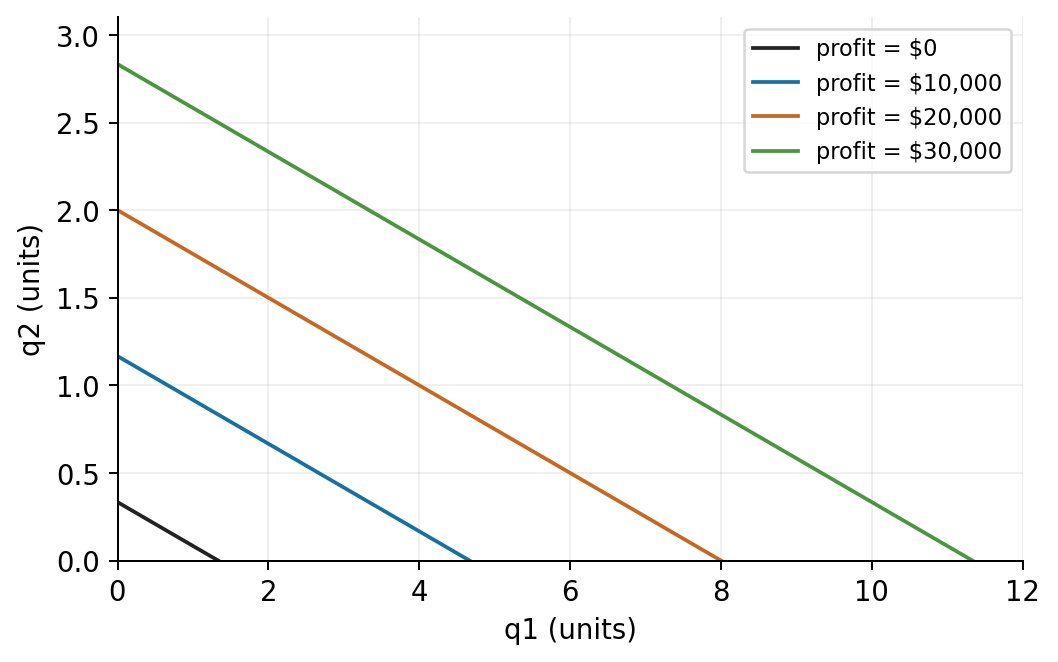
\includegraphics[width=.74\linewidth]{graphs/answer-12-3-47.png}\end{center}
